\documentclass{article}
%babel
\usepackage[romanian]{babel}
%
\usepackage{graphicx}%dorim să importăm grafică
%titlu
\title{L3: studiul unui circuit $RC$ serie}
\author{Student}
\begin{document}
\maketitle
\begin{abstract}
Se studiază un circuit $RC$ serie. 
\end{abstract}
\section{Introducere}
Se aplică teorema lui Kirchhoff și legile lui Ohm. Pentru simboluri folosim litera grecească $\Omega$ care diferă de $\omega$. Ambele pot fi afișate doar în mod matematic, cu comenzile \verb+$\Omega$+ sau \verb+$\omega$+.
\section{Studiul circuitului $RC$ serie}
Se dă circuitul din figura\ref{fig:rc}. \par
\begin{figure}[htpb]
\centering
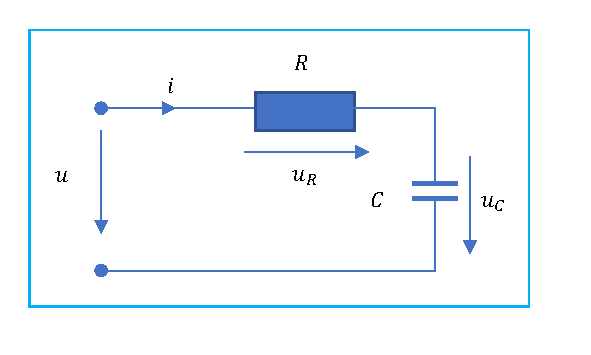
\includegraphics[scale=0.8]{poza_RC.pdf}
\caption{Circuitul $RC$ serie.}\label{fig:rc}
\end{figure}
Aplicând relațiile
\begin{eqnarray}
u&=&u_R+u_C\\
u_R&=&Ri\\
i&=&C\frac{du_C}{dt}
\end{eqnarray}
rezultă ecuația diferențială în regim tranzitoriu
\begin{equation}
RC\frac{du_C}{dt}+u_C=u.
\end{equation}
Valorile parametrilor de circuit sunt specificate în tabelul următor.
\begin{table}[htpb]
\centering
\begin{tabular}{cc}
\emph{Element}&\emph{Valoare}\\\hline
$R [\Omega]$&2\\
$C[F]$&0.5\\\hline
\end{tabular}
\caption{Valorile elementelor circuitului din figura \ref{fig:rc}.}
\end{table}

\end{document}